\chapter{\sffamily Empirical dynamical emulators}

{\bfseries\sffamily Concept.} To extend the formalism that we developed in previous chapters to enable the empirical emulation of real-world data in a probabilistic way. This technique should enable a researcher to model complex dynamical trends in the data very well; at the cost of making the abstract interpretation of the model less immediately comprehensible than the statistical inference models in some proceeding chapters. As our generalised framework applies to a wide variety stochastic phenomena, our emulator will be applicable to a great breadth of data modeling problems as well. We will also explore some examples which illustrate how our empirical emulator should be applied in practice and then follow this up with how the code is designed and implemented as part of a new software package called `learnadex'. For the mathematically-inclined, this chapter will take a detailed look at how our formalism can be extended to focus on probabilistic dynamical process emulation. For the programmers, the software described in this chapter lives in the public Git repository: \href{https://github.com/umbralcalc/learnadex}{https://github.com/umbralcalc/learnadex}.

\section{\sffamily Probabilistic formalism}

The key distinction between the methods that we will develop in this chapter and the ones in the proceeding chapters is in their utility when faced with the problem of attempting to model real-world data. In the proceeding chapter, we shall describe some powerful techniques that can be used most effectively when the researcher is aware of the family of models that generated the data. In the present chapter, we will go into the details of how a more `empirical' approach can be derived for dynamical process modeling in a probabilistic framework which locally adapts the model to the data through time. 

While we think that it's worth going into some mathematical detail to give a better sense of where our formalism comes from; we want to emphasise that the framework we discuss here is not especially new to the technical literature. Our overall framework draws on influences from Empirical Dynamical Modeling (EDM)~\cite{sugihara1990nonlinear}, some classic nonparametric local regression techniques --- such as LOWESS/Savitzky-Golay filtering~\cite{savitzky1964smoothing} --- and perhaps Gaussian processes~\cite{murphy2012machine} as well. The novelties here, instead, lie more in the specifics of how we combine some of these ideas together when referencing the stochadex formalism, and how this manifests in designing more generally-applicable software for the user.

Before we are able to develop this empirical emulator, we need to return to the stochadex formalism that we introduced in the first chapter of this book. As we discussed at that point; this formalism is appropriate for sampling from nearly every stochastic phenomenon that one can think of. However, when trying robustly assess how far a model is from accurately describing a set of real-world data, trying to use only generated samples of the model process can be diffcult. Instead, in this section, we are going to extend this formalism to look at how probability theory can help with this data comparison problem in a systematic way.

So, how do we begin? In the first chapter, we defined the general stochastic process with the formula $X^{i}_{{\sf t}+1} = F^{i}_{{\sf t}+1}(X',z,{\sf t})$. This equation also has an implicit \emph{master equation} associated to it that fully describes the time evolution of the \emph{probability density function} $P_{{\sf t}+1}(x)$ of the next matrix row being $x=X_{{\sf t}+1}$. This can be written as
%%
\begin{align}
P_{{\sf t}+1}(x) &= \frac{1}{{\sf t}}\sum_{{\sf t}'=0}^{{\sf t}}\int_{\omega_{{\sf t}'}}{\rm d}x' P_{{\sf t}'}(x') P_{({\sf t}+1){\sf t}'}(x\vert x') \label{eq:master-x-cont} \,,
\end{align}
%%
where at the moment we are assuming the state space is continuous in each dimension and $P_{({\sf t}+1){\sf t}'}(x\vert x')$ is the conditional probability that the matrix row at time $({\sf t}+1)$ will be $x=X_{{\sf t}+1}$ given that the row at time ${\sf t}'$ was $x'=X_{{\sf t}'}$. This is a very general equation which should almost always apply to any continuous stochastic phenomenon we want to study in due course. To try and understand what this equation is saying we find it's helpful to think of an iterative relationship between probabilities; each of which is connected by their relative conditional probabilities. This kind of thinking is also illustrated in Fig.~\ref{fig:master-eqn}. Let's say we also wanted to program what this equation is saying as a function in Go. Using a Monte Carlo approximation for the integral domain, the code might look something like this.

\begin{lstlisting}[language=Go]
type StateVector  []float64

// returns a random draw of the possible state vectors at this timestep
func RandomPossibleStateVectors(timeStepNumber int) []StateVector {
    // return a slice of randomly-drawn possible state vectors 
    // corresponding to the integral domain at this timestep
}

// returns the conditional probability of the state vector at this timestep 
// given the value that the state vector had on a previous timestep
func StateVectorConditionalProbability(
    stateVector StateVector,
    timeStepNumber int,
    previousStateVector StateVector,
    previousTimeStepNumber int,
) float64 {
    // return the conditional probability value
}

// returns the probability of the state vector at this timestep
func StateVectorProbability(
    stateVector StateVector, 
    timeStepNumber int,
) float64 {
    prob := 0.0
    // loop over all the possible previous timesteps
    for t := 0; t < timeStepNumber; t++ {
        // loop over the randomly-drawn possible state vectors 
        // for this previous timestep
        possibleStateVectors := RandomPossibleStateVectors(t)
        for _, possibleStateVector := range possibleStateVectors {
            // note the recursion
            prob += StateVectorProbability(possibleStateVector, t)*
                StateVectorConditionalProbability(
                    stateVector,
                    timeStepNumber,
                    possibleStateVector, 
                    t,
                )
        }
        // normalisation for the Monte Carlo integration
        prob /= float64(len(possibleStateVectors))
    }
    // timestep normalisation
    prob /= float64(timeStepNumber)
    return prob
}
\end{lstlisting}

The factor of $1/{\sf t}$ in Eq.~(\ref{eq:master-x-cont}) is a normalisation factor --- this just normalises the sum of all probabilities to 1 given that there is a sum over ${\sf t}'$. Note that, if the process is defined over continuous time, we would need to replace 
%%
\begin{align}
\frac{1}{{\sf t}}\sum_{{\sf t}'=0}^{{\sf t}} \rightarrow \frac{1}{t({\sf t})}\sum_{{\sf t}'=0}^{{\sf t}}\delta t({\sf t}') \,.
\end{align}
%% 
But what is $\omega_{\sf t}$? You can think of this as just the domain of possible $x'$ inputs into the integral which will depend on the specific stochastic process we are looking at.

\begin{figure}[h]
\centering
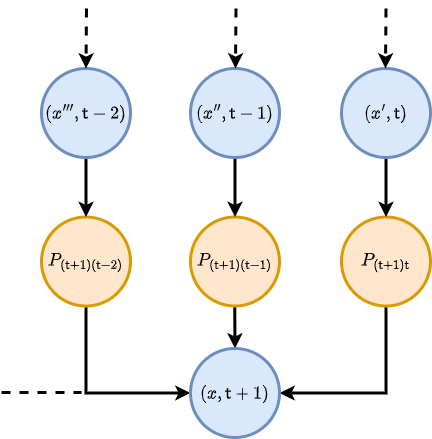
\includegraphics[width=8cm]{images/master-eq-graph.drawio.png}
\caption{Graph representation of Eq.~(\ref{eq:master-x-cont}).}
\label{fig:master-eqn}
\end{figure} 

If we wanted to compute the mean of the distribution $M_{{\sf t}+1}$ in Eq.~(\ref{eq:master-x-cont}), it would be straightforward to just multiply both sides of the expression by $x$ and integrate over ${\rm d}x$ in the $\omega_{{\sf t}}$ domain. However, there is another similar expression for the mean that we can derive under certain conditions which will be valuable to us when developing the empirical emulator. If the probability distribution is \emph{stationary} --- meaning that $P_{{\sf t}'}(x)=P_{{\sf t}''}(x)$ for all ${\sf t}'$ and ${\sf t}''$ --- it's possible to derive\footnote{To see that this is true, first note that the joint distribution $P_{({\sf t}+1){\sf t}'}(x,x')=P_{({\sf t}+1){\sf t}'}(x\vert x')P_{{\sf t}'}(x')$. Secondly, note that joint distributions always allow variable swaps trivially like this $P_{({\sf t}+1){\sf t}'}(x,x')=P_{{\sf t}'({\sf t}+1)}(x',x)$. Then, lastly, note that stationarity of $P_{{\sf t}+1}(x)=P_{{\sf t}'}(x)$ means 
$$M_{{\sf t}+1}=\int {\rm d}x\int {\rm d}x' \, x\,P_{({\sf t}+1){\sf t}'}(x,x')=\int {\rm d}x\int {\rm d}x'  \, x\, P_{{\sf t}'({\sf t}+1)}(x,x')=\int {\rm d}x\int {\rm d}x'  \, x\, P_{({\sf t}+1){\sf t}'}(x',x)\,,$$
where we've used the trivial variable swap to get to the last equality, and the domain references $\omega_{{\sf t}'}$ in the integrals are implicitly defined.} 
%%
\begin{align}
M_{{\sf t}+1} = \int_{\omega_{{\sf t}+1}}{\rm d}x \,x\,P_{{\sf t}+1}(x) &= \frac{1}{{\sf t}}\sum_{{\sf t}'=0}^{{\sf t}}\int_{\omega_{{\sf t}'}}{\rm d}x'\int_{\omega_{{\sf t}+1}}{\rm d}x \, x' \, P_{{\sf t}'}(x') P_{({\sf t}+1){\sf t}'}(x\vert x') \label{eq:stationary-mean-estimator}\,.
\end{align}
%%

In order to encode higher-order out-of-time-order correlations; we can also consider using the statistical moments computed from joint distributions like these
%%
\begin{align}
P_{({\sf t}+1){\sf t}'}(x, x') &= P_{({\sf t}+1){\sf t}'}(x\vert x')P_{{\sf t}'}(x') \label{eq:2nd-joint-dist}\\
P_{({\sf t}+1){\sf t}'{\sf t}''}(x, x', x'') &= P_{({\sf t}+1){\sf t}'{\sf t}''}(x\vert x', x'')P_{{\sf t}'{\sf t}''}(x'\vert x'')P_{{\sf t}''}(x'') \label{eq:3rd-joint-dist}\,.
\end{align}
%%
For example, Eq.~(\ref{eq:2nd-joint-dist}) would apply if we wanted to retrieve the out-of-time-order pairwise correlations between $x$ at timestep ${\sf t}+1$ and $x'$ at timestep ${\sf t}'$. Using this pairwise relationship we can also derive an equation for the stationary out-of-time-order covariance matrix elements
%%
\begin{align}
C_{({\sf t}+1){\sf t}'}^{ij} &= \frac{1}{{\sf t}}\sum_{{\sf t}'=0}^{{\sf t}}\int_{\omega_{{\sf t}'}}{\rm d}x'\int_{\omega_{{\sf t}+1}}{\rm d}x \,(x-M_{{\sf t}+1})^i(x'-M_{{\sf t}'})^j P_{({\sf t}+1){\sf t}'}(x, x') \label{eq:stationary-covariance-estimator} \,.
\end{align}
%%

What other processes can be described by Eq.~(\ref{eq:master-x-cont})? For Markovian phenomena, the equation no longer depends on timesteps older than the immediately previous one, hence the expression reduces to just
%%
\begin{align}
P_{{\sf t}+1}(x) &= \int_{\omega_{\sf t}}{\rm d}x' P_{\sf t}(x') P_{({\sf t}+1){\sf t}}(x\vert x') \label{eq:master-x-cont-markov} \,.
\end{align}
%%
An analog of Eq.~(\ref{eq:master-x-cont}) exists for discrete state spaces as well. We just need to replace the integral with a sum and the schematic would look something like this
%%
\begin{align}
P_{{\sf t}+1}(x) &= \frac{1}{{\sf t}}\sum_{{\sf t}'=0}^{\sf t}\sum_{\omega_{{\sf t}'}} P_{{\sf t}'}(x') P_{({\sf t}+1){\sf t}'}(x \vert x') \label{eq:master-x-disc} \,,
\end{align}
%%
where we note that the $P$'s in the expression above all now refer to \emph{probability mass functions}. In the even-simpler case where $x$ is just a vector of binary `on' or `off' states, Eq.~(\ref{eq:master-x-disc}) reduces to
%%
\begin{align}
P^i_{{\sf t}+1} &= \frac{1}{{\sf t}}\sum_{{\sf t}'=0}^{\sf t} \sum_{j=1}^d P^j_{{\sf t}'} P^{ij}_{({\sf t}+1){\sf t}'} = \frac{1}{{\sf t}}\sum_{{\sf t}'=0}^{\sf t} \sum_{j=1}^d \big[ P^j_{{\sf t}'} A^{ij}_{({\sf t}+1){\sf t}'} + (1-P^j_{{\sf t}'}) B^{ij}_{({\sf t}+1){\sf t}'} \big] \label{eq:master-x-disc-binary}\,,
\end{align}
%% 
where $P^i_{{\sf t}'}$ now represents the probability that element $x^i=1$ (is `on') at time ${\sf t}'$. The matrices $A$ and $B$ are defined as conditional probabilities where the previous state in time $P^j_{{\sf t}'}$ was either `on' or `off', respectively.

In this section, we looked into how the mathematical formalism used in the stochadex could be extended with probability theory. Now that we have more of a sense of how this formalism works, we are ready to move on to designing the algorithms for our emulator. So let's go!

\section{\sffamily Emulator algorithms}

Helpful to write the basic structure of algorithm out in Go.

\section{\sffamily Software design}

